\documentclass[11pt,aspectratio=169]{beamer}
\usepackage{imaxbeamer}
\usetikzlibrary{patterns}

\title[F25 -- Endelig volum i 2D]{Forelesning 25\\ Endelig volum-metoden i 2D}
\subtitle{Kompendium §3.6}
\author{IMAx3012 / IMAA3012 -- Matematikk 3B}
\date{}

\tikzset{
  nodept/.style={circle, fill=black, inner sep=0pt, minimum size=1.8mm},
}

\begin{document}

\begin{frame}
\titlepage
\end{frame}

\begin{frame}{I dag}
\begin{remb}{Fra F23 og F24 (1D)}
\[
a_P\phi_P = a_W\phi_W + a_E\phi_E + S^u, \qquad a_P = a_W + a_E - S_P
\]
Kjent temperatur på randen: kutt koblingen, $S_P \to S_P - 2\Gamma A/\delta x$, $S^u \to S^u + (2\Gamma A/\delta x)\phi_B$. \quad Kjent fluks: $S^u \to S^u + q_BA$.
\end{remb}
\begin{enumerate}
\item Fra 1D til 2D: fire naboer og fire flater.
\item Randceller og hjørneceller.
\item Sammenhengen med fempunktsformelen fra F21.
\item Nummerering av cellene og matrisen $L$ -- også med \texttt{np.kron}.
\item Eksempel: plate med varmefluks inn fra vest (kompendiet).
\end{enumerate}
\medskip
Kode til eksemplene finnes i \texttt{F25\_EVM\_2D.ipynb} -- se gjerne på den.
\end{frame}

\section{Fra 1D til 2D}

\begin{frame}{Kontrollvolum i 2D: fire naboer og fire flater}
\begin{columns}[c]
\begin{column}{0.45\textwidth}
\centering
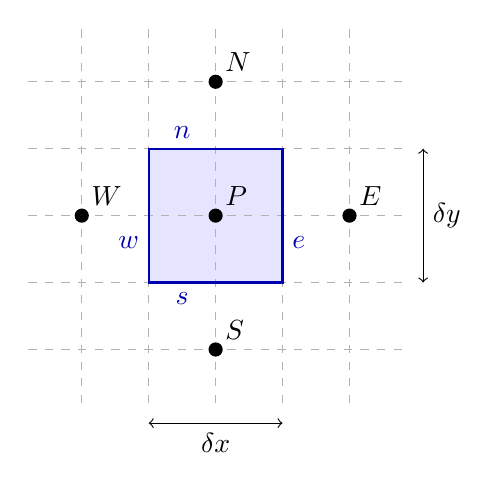
\begin{tikzpicture}[scale=0.85]
\fill[blue!10] (1.5,1.5) rectangle (3.5,3.5);
\foreach \v in {0.5,1.5,2.5,3.5,4.5} {
  \draw[gray!60, dashed] (\v,-0.3) -- (\v,5.3);
  \draw[gray!60, dashed] (-0.3,\v) -- (5.3,\v);
}
\draw[thick, blue!70!black] (1.5,1.5) rectangle (3.5,3.5);
\foreach \p/\x/\y in {P/2.5/2.5, W/0.5/2.5, E/4.5/2.5, S/2.5/0.5, N/2.5/4.5}
  {\node[nodept] at (\x,\y) {}; \node[above right] at (\x,\y) {$\p$};}
\node[left, blue!70!black] at (1.5,2.1) {$w$};
\node[right, blue!70!black] at (3.5,2.1) {$e$};
\node[below, blue!70!black] at (2.0,1.5) {$s$};
\node[above, blue!70!black] at (2.0,3.5) {$n$};
\draw[<->] (1.5,-0.6) -- (3.5,-0.6) node[midway, below] {$\delta x$};
\draw[<->] (5.6,1.5) -- (5.6,3.5) node[midway, right] {$\delta y$};
\end{tikzpicture}
\end{column}
\begin{column}{0.53\textwidth}
\[
\frac{\partial}{\partial x}\Big(\Gamma\frac{\partial\phi}{\partial x}\Big) + \frac{\partial}{\partial y}\Big(\Gamma\frac{\partial\phi}{\partial y}\Big) + S = 0
\]
\begin{itemize}
\item Naboer $W, E, S, N$; flater $w, e, s, n$.
\item Dybde $t$ i $z$-retning (en plate):
\[
A_w = A_e = \delta y\,t, \qquad A_s = A_n = \delta x\,t,
\]
\[
\Delta V = \delta x\,\delta y\,t .
\]
\item Ingenting nytt i metoden -- bare \emph{to flater til}.
\end{itemize}
\end{column}
\end{columns}
\end{frame}

\begin{frame}{Integrer over kontrollvolumet}
Divergenssetningen gjør volumintegralet om til fluks over de fire flatene:
\[
\underbrace{\Gamma_eA_e\Big(\frac{\partial\phi}{\partial x}\Big)_e - \Gamma_wA_w\Big(\frac{\partial\phi}{\partial x}\Big)_w}_{\text{fluks i } x\text{-retning}}
+ \underbrace{\Gamma_nA_n\Big(\frac{\partial\phi}{\partial y}\Big)_n - \Gamma_sA_s\Big(\frac{\partial\phi}{\partial y}\Big)_s}_{\text{fluks i } y\text{-retning}}
+ \overline S\,\Delta V = 0
\]
Lineær tilnærming mellom nodene, og $\overline S\,\Delta V = S^u + S_P\phi_P$:
\begin{oppsumb}{Den diskrete ligningen i 2D}
\[
a_P\phi_P = a_W\phi_W + a_E\phi_E + a_S\phi_S + a_N\phi_N + S^u, \qquad a_P = a_W + a_E + a_S + a_N - S_P
\]
\[
a_W = \frac{\Gamma_wA_w}{\delta x_{WP}}, \quad a_E = \frac{\Gamma_eA_e}{\delta x_{PE}}, \quad a_S = \frac{\Gamma_sA_s}{\delta y_{SP}}, \quad a_N = \frac{\Gamma_nA_n}{\delta y_{PN}}
\]
\end{oppsumb}
\end{frame}

\begin{frame}{Randceller og hjørneceller}
\begin{columns}[c]
\begin{column}{0.40\textwidth}
\centering
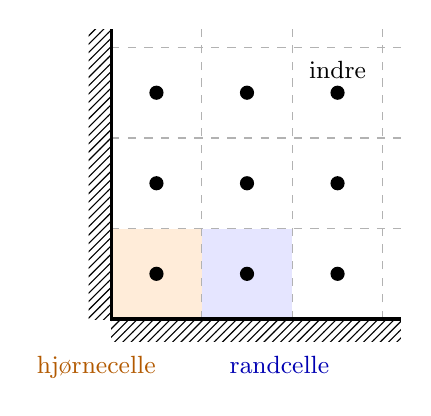
\begin{tikzpicture}[scale=1.15]
\fill[orange!15] (0,0) rectangle (1,1);
\fill[blue!10] (1,0) rectangle (2,1);
\foreach \v in {1,2,3} {\draw[gray!60, dashed] (\v,0) -- (\v,3.2); \draw[gray!60, dashed] (0,\v) -- (3.2,\v);}
\draw[very thick] (3.2,0) -- (0,0) -- (0,3.2);
\fill[pattern=north east lines] (-0.25,0) rectangle (0,3.2);
\fill[pattern=north east lines] (0,-0.25) rectangle (3.2,0);
\foreach \i in {0.5,1.5,2.5} \foreach \j in {0.5,1.5,2.5} \node[nodept] at (\i,\j) {};
\node[orange!70!black, font=\small, anchor=north east] at (0.6,-0.3) {hjørnecelle};
\node[blue!70!black, font=\small, anchor=north west] at (1.2,-0.3) {randcelle};
\node[font=\small, anchor=south] at (2.5,2.55) {indre};
\end{tikzpicture}
\end{column}
\begin{column}{0.58\textwidth}
Som i 1D: \textbf{kutt koblingen} mot veggen, og legg bidraget i $S^u$ og $S_P$.
\begin{itemize}
\item \textbf{Kjent temperatur} $\phi_B$ (avstand $\delta/2$):
\[
a_{\text{vegg}} = 0, \qquad \begin{aligned} S_P &\to S_P - \frac{2\Gamma A}{\delta},\\ S^u &\to S^u + \frac{2\Gamma A}{\delta}\,\phi_B \end{aligned}
\]
\item \textbf{Kjent fluks} $q_B$ inn: \quad $a_{\text{vegg}}=0$, \quad $S^u \to S^u + q_B A$.
\item \textbf{Isolert vegg:} $q_B=0$ -- ingen bidrag.
\end{itemize}
\begin{remb}{Hjørneceller}
En hjørnecelle ligger inntil \emph{to} vegger, og får ett bidrag fra \emph{hver} av dem.
\end{remb}
\end{column}
\end{columns}
\end{frame}

\begin{frame}{Sammenheng med fempunktsformelen (F21)}
\begin{columns}[c]
\begin{column}{0.55\textwidth}
Konstant $\Gamma$, uniformt gitter $\delta x = \delta y = h$, $t=1$:
\[
a_W = \frac{\Gamma A_w}{\delta x} = \frac{\Gamma\,h}{h} = \Gamma,
\]
og tilsvarende $a_E=a_S=a_N=\Gamma$.

\medskip
Indre celle uten kilde:
\[
4\phi_P = \phi_W + \phi_E + \phi_S + \phi_N
\]
-- nøyaktig \textbf{fempunktsformelen} og Jacobi-formelen fra F21!
\end{column}
\begin{column}{0.43\textwidth}
\begin{remb}{Forskjellen ligger ved randen}
Med kjent randtemperatur:
\begin{itemize}
\item randcelle: $a_P = 3 + 2 = 5$,
\item hjørnecelle: $a_P = 2 + 2 + 2 = 6$
\end{itemize}
(ganger $\Gamma$). Avstanden til veggen er bare $h/2$ -- som tallet $3$ i stedet for $2$ i 1D.
\end{remb}
Og EVM tåler uten videre kjent fluks, variabel $\Gamma$ og ikke-uniforme gitre.
\end{column}
\end{columns}
\end{frame}

\begin{frame}{Nummerering av cellene -- og matrisen $L$}
\begin{columns}[c]
\begin{column}{0.56\textwidth}
\small
Nummerer cellene \textbf{rad for rad}: celle $(i,j)$ får nummeret
\[
p = (j-1)\,m + i, \qquad i = 1,\ldots,m, \quad j=1,\ldots,n .
\]
Da er naboene \vspace{-2mm}
\[
W = p-1, \quad E = p+1, \quad S = p-m, \quad N = p+m .
\]
\begin{itemize}
\item Rad $p$ i $L$: $a_P$ på diagonalen, $-a_W,-a_E,-a_S,-a_N$ i kolonnene til naboene. $F_p = S^u$.
\item \textbf{Fem diagonaler} -- samme struktur som i F21 og øving 6.
\item I Python (fra 0): \texttt{p = j*m + i},\\ \texttt{U = np.reshape(u, (n, m))}.
\end{itemize}
\end{column}
\begin{column}{0.42\textwidth}
\centering
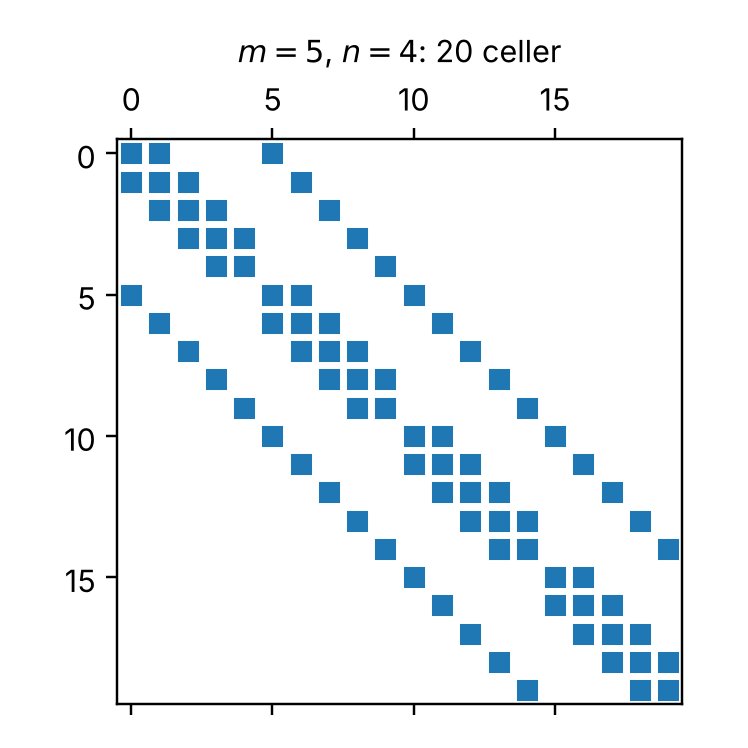
\includegraphics[width=0.9\textwidth]{assets/spy.png}
\end{column}
\end{columns}
\end{frame}

\begin{frame}[fragile]{Samme matrise med \texttt{np.kron} -- som i øving 6}
\begin{columns}[T]
\begin{column}{0.47\textwidth}
\footnotesize
Uniformt gitter: $x$-koblingene er like i hver rad, $y$-koblingene like i hver kolonne. Vi trenger bare \textbf{1D-matrisen fra F23} i hver retning:
\[
L_m = \frac{1}{\delta x}\begin{bmatrix} 3 & -1 & & \\ -1 & 2 & \ddots & \\ & \ddots & \ddots & -1 \\ & & -1 & 3\end{bmatrix}
\quad (m\times m),
\]
og $L_n$ ($n\times n$) med $\delta y$. Flatearealene gir vektene:
\[
L = k\,t\,\Big(\underbrace{\delta y\;I_n\otimes L_m}_{W,\,E \text{ i hver rad}} \;+\; \underbrace{\delta x\;L_n\otimes I_m}_{S,\,N \text{ i hver kolonne}}\Big)
\]
Diagonal ($\delta x=\delta y$): indre $2+2=4$, rand $3+2=5$, hjørne $3+3=6$.\\[1mm] \textbf{Nøyaktig samme $L$ og $F$ som løkken} (sjekket i notatboken).
\end{column}
\begin{column}{0.51\textwidth}
\begin{lstb}[Python-kode]
\begin{lstlisting}[basicstyle=\ttfamily\scriptsize]
# 1D-matrisene fra F23 (k*A = 1)
x, dx, Lm = evm_1d_matrise(Lx, m)
y, dy, Ln = evm_1d_matrise(Ly, n)
Im, In = np.eye(m), np.eye(n)

L = k*t*(deltay*np.kron(In, Lm)
       + deltax*np.kron(Ln, Im))

# randledd, f.eks. nordveggen:
e_n = np.zeros(n); e_n[-1] = 1
F = k*t*deltax*np.kron(e_n, T_N)/dy[-1]
# (+ tilsvarende for S, V, H)

u = la.solve(L, F)
U = np.reshape(u, (n, m))
\end{lstlisting}
\end{lstb}
\end{column}
\end{columns}
\end{frame}

\section{Eksempel}

\begin{frame}{Eksempel: plate med varmefluks inn fra vest}
\begin{columns}[c]
\begin{column}{0.42\textwidth}
\centering
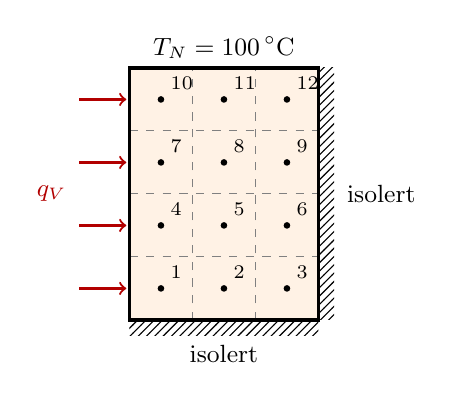
\begin{tikzpicture}[scale=0.8]
\fill[orange!10] (0,0) rectangle (3,4);
\foreach \x in {1,2} \draw[gray, dashed] (\x,0) -- (\x,4);
\foreach \y in {1,2,3} \draw[gray, dashed] (0,\y) -- (3,\y);
\draw[very thick] (0,0) rectangle (3,4);
\foreach \j in {1,...,4} \foreach \i in {1,...,3} {
  \pgfmathtruncatemacro{\p}{(\j-1)*3+\i}
  \fill (\i-0.5,\j-0.5) circle (1.5pt);
  \node[font=\scriptsize, anchor=south west] at (\i-0.5,\j-0.5) {\p};
}
\foreach \y in {0.5,1.5,2.5,3.5} \draw[->, thick, red!70!black] (-0.8,\y) -- (-0.05,\y);
\node[left, red!70!black, align=right, font=\small] at (-0.85,2) {$q_V$};
\fill[pattern=north east lines] (0,-0.25) rectangle (3,0);
\node[below, font=\small] at (1.5,-0.25) {isolert};
\fill[pattern=north east lines] (3,0) rectangle (3.25,4);
\node[right, font=\small] at (3.3,2) {isolert};
\node[above, font=\small] at (1.5,4) {$T_N = 100\,^\circ$C};
\end{tikzpicture}
\end{column}
\begin{column}{0.56\textwidth}
\begin{itemize}
\item Plate $0.3\,\text{m}\times 0.4\,\text{m}$, tykkelse $t = 1$ cm, $\kappa = 1000$ W/(m K).
\item Vest: varmefluks inn $q_V = 500$ kW/m$^2$.
\item Sør og øst: isolert. \quad Nord: $T_N = 100\,^\circ$C.
\item $3\times4$ kontrollvolum: $\delta x = \delta y = 0.1$ m.
\end{itemize}
Alle indre koblinger:
\[
\frac{\kappa A}{\delta x} = \frac{1000\cdot 0.1\cdot 0.01}{0.1} = 10 .
\]
\begin{itemize}
\item Vestvegg: $S^u \to S^u + q_VA_w = S^u + 500$.
\item Nordvegg: $S_P \to S_P - 20$, $S^u \to S^u + 20\cdot 100$.
\end{itemize}
\end{column}
\end{columns}
\end{frame}

\begin{frame}{Koeffisientene}
\centering\small
\begin{tabular}{lccccccc}
\toprule
Celle & $a_W$ & $a_E$ & $a_S$ & $a_N$ & $S^u$ & $S_P$ & $a_P$ \\
\midrule
1 (hjørne sørvest) & 0 & 10 & 0 & 10 & 500 & 0 & 20 \\
2 (sørvegg) & 10 & 10 & 0 & 10 & 0 & 0 & 30 \\
3 (hjørne sørøst) & 10 & 0 & 0 & 10 & 0 & 0 & 20 \\
4, 7 (vestvegg) & 0 & 10 & 10 & 10 & 500 & 0 & 30 \\
5, 8 (indre) & 10 & 10 & 10 & 10 & 0 & 0 & 40 \\
6, 9 (østvegg) & 10 & 0 & 10 & 10 & 0 & 0 & 30 \\
10 (hjørne nordvest) & 0 & 10 & 10 & 0 & $500+2000$ & $-20$ & 40 \\
11 (nordvegg) & 10 & 10 & 10 & 0 & 2000 & $-20$ & 50 \\
12 (hjørne nordøst) & 10 & 0 & 10 & 0 & 2000 & $-20$ & 40 \\
\bottomrule
\end{tabular}
\begin{remb}{Les av}
De isolerte veggene gir bare $a=0$. Hjørne 10 får bidrag fra \emph{både} vest- og nordveggen.
\end{remb}
\end{frame}

\begin{frame}{Løsningen -- og energibalansen}
\begin{columns}[c]
\begin{column}{0.40\textwidth}
\centering
Temperatur i $^\circ$C (nord øverst):\\[2mm]
\begin{tabular}{|c|c|c|}
\hline
146.3 & 129.7 & 124.0 \\ \hline
205.6 & 178.2 & 166.2 \\ \hline
242.3 & 211.2 & 196.5 \\ \hline
260.0 & 227.8 & 212.2 \\ \hline
\end{tabular}
\\[3mm]
\small Varmest i sørvest -- lengst unna den kalde nordveggen.
\end{column}
\begin{column}{0.58\textwidth}
\begin{oppsumb}{Energibalansen}
Inn gjennom vest: \quad $4\cdot 500 = 2000$ W.\\[1mm]
Ut gjennom nord: \quad $\displaystyle\sum 20\,(T_P - 100)$
\[
= 20\,(46.3 + 29.7 + 24.0) = 2000 \text{ W}.
\]
\end{oppsumb}
\begin{itemize}
\item Eksakt -- selv på et grovt gitter: fluksen ut av én celle er fluksen inn i neste.
\item Sør og øst er isolert, så all varmen \emph{må} ut gjennom nord.
\end{itemize}
\end{column}
\end{columns}
\end{frame}

\begin{frame}{Finere gitter}
\begin{columns}[c]
\begin{column}{0.40\textwidth}
\centering
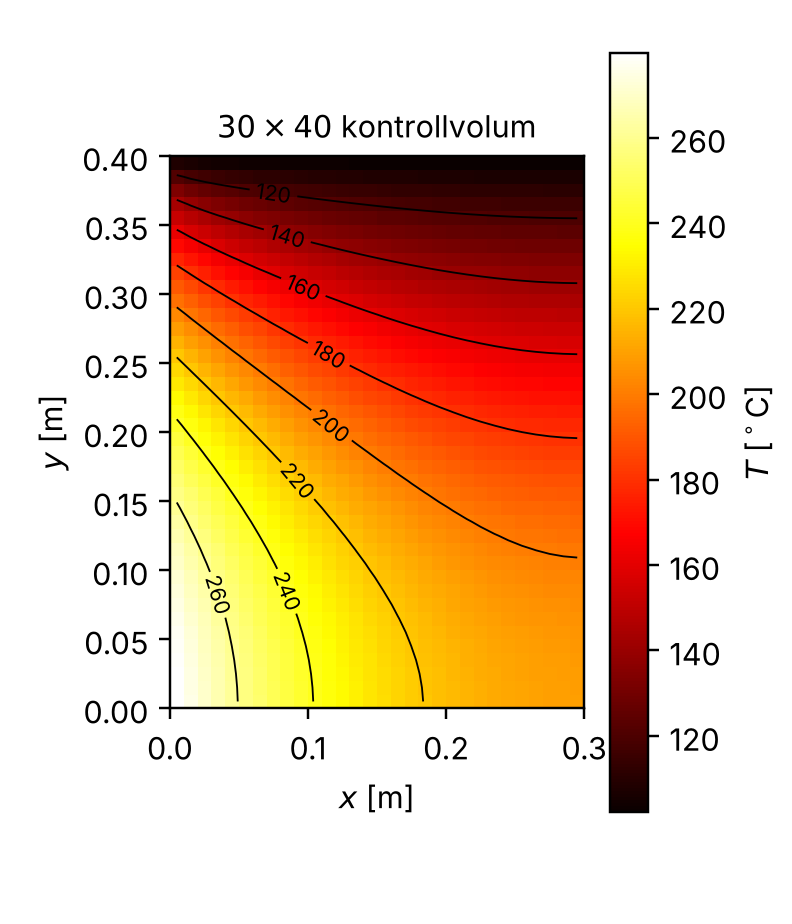
\includegraphics[height=0.78\textheight]{assets/plate_varmekart.png}
\end{column}
\begin{column}{0.58\textwidth}
\small
\begin{tabular}{ccc}
\toprule
Gitter & Høyeste $T$ & Inn $-$ ut \\
\midrule
$3\times 4$ & $260.0\,^\circ$C & $0$ \\
$6\times 8$ & $270.6\,^\circ$C & $0$ \\
$12\times 16$ & $276.3\,^\circ$C & $0$ \\
$24\times 32$ & $279.3\,^\circ$C & $0$ \\
$48\times 64$ & $280.9\,^\circ$C & $0$ \\
\bottomrule
\end{tabular}
\begin{itemize}
\item Temperaturfordelingen blir mer nøyaktig; energibalansen er eksakt på \emph{alle} gitre.
\item Isotermene står vinkelrett på de isolerte veggene: $\partial T/\partial n = 0$.
\item Mot en eksakt løsning (Laplace på enhetskvadratet): feilen er $O(h^2)$, som i 1D.
\end{itemize}
\end{column}
\end{columns}
\end{frame}

\begin{frame}{Oppsummering}
\begin{oppsumb}{Endelig volum i 2D}
\begin{enumerate}
\item Hvert kontrollvolum har fire naboer og fire flater, med $A_w=A_e=\delta y\,t$ og $A_s=A_n=\delta x\,t$.
\item $a_P\phi_P = a_W\phi_W + a_E\phi_E + a_S\phi_S + a_N\phi_N + S^u$, \quad $a_P = a_W+a_E+a_S+a_N - S_P$.
\item Randceller: kutt koblingen og legg bidraget i $S^u$ og $S_P$ -- akkurat som i 1D. Hjørneceller får to bidrag.
\item Nummerer rad for rad: matrisen får fem diagonaler.
\end{enumerate}
\end{oppsumb}
\begin{itemize}
\item Indre celler: samme ligning som fempunktsformelen. Forskjellen er randbehandlingen.
\item Metoden er konservativ: energibalansen stemmer eksakt.
\end{itemize}
\end{frame}

\begin{frame}{Koding: \texttt{F25\_EVM\_2D.ipynb}}
\begin{enumerate}
\item \textbf{Gitteret} som i F23, i begge retninger, og nummereringen \texttt{p = j*m + i}.
\item \textbf{En 2D-løser} \texttt{evm\_2d}: går gjennom cellene og setter opp \texttt{L} og \texttt{F} -- slik vi gjør for hånd. Randbetingelser \texttt{"T"} eller \texttt{"fluks"} på hver vegg.
\item \textbf{Eksempelet fra kompendiet:} koeffisienter, løsning og energibalanse.
\item \textbf{Varmekart} på et finere gitter.
\item \textbf{Konvergens} mot en eksakt løsning av Laplace-ligningen.
\item \textbf{Matrisen:} fem diagonaler -- og den samme matrisen bygget med \texttt{np.kron}, som i øving 6.
\end{enumerate}
\begin{remb}{Prøv selv (i notatboken)}
Varmekilde i platen \;$\cdot$\; østveggen med kjent temperatur \;$\cdot$\; Gauss-Seidel over cellene.
\end{remb}
\end{frame}

\begin{frame}{Neste gang: F26 -- tidsavhengige problemer}
\begin{nestefb}
\begin{itemize}
\item Integrer over kontrollvolumet \emph{og} over et tidsintervall.
\item Eksplisitt skjema -- med samme $L$ og $F$ som i det stasjonære problemet.
\item Stabilitet: hvorfor randcellene gir det strengeste kravet.
\item Oppsummering av kapittel 3.
\end{itemize}
\end{nestefb}
\end{frame}

\end{document}
